\section{Numerical simulations}\label{sec:numerical}
We follow the presentation in Section 4 of \citet{haque11}, beginning with the model inputs and then pairing equilibrium branches with phase portraits and time-dependent checks. The examples in Table~\ref{tab:constructed} were constructed from the analytical conditions, with density and time units chosen for each example. Section~\ref{sec:literature-cases} varies prey growth over values reported in the literature.

\begin{table}[!htbp]\centering
\caption{Dimensional inputs for the constructed cases. Each one-parameter path holds all other entries fixed. The values of \(m\), \(k\) and \(\beta\) in a two-parameter case are varied only as indicated.}
\label{tab:constructed}
\begin{tabular}{@{}lccccccc@{}}
\toprule
Case & \(r\) & \(k\) & \(\alpha\) & \(m\) & \(\beta\) & \(e\) & \(d\) \\ \midrule
Invasion & 1 & 1 & 2 & varied & 1 & 1 & 1\\
Bistability & 1 & 1 & 10 & 3 & 1 & \(70/3\) & \(7/5\)\\
Cusp & 1 & 1 & 10 & varied & varied & \(70/3\) & \(7/5\)\\
Predation Hopf & 1 & 1 & 10 & varied & \(6/25\) & 1 & 2\\
Enrichment Hopf & 1 & varied & 10 & \(53/10\) & \(9/53\) & 1 & \(371/180\)\\
Bogdanov--Takens & 1 & varied & 10 & varied & \(12/85\) & 1 & \(17/12\)\\
Unique cycle & 1 & 1 & 10 & 12 & 1 & \(77/48\) & \(7/2\)\\
\bottomrule
\end{tabular}
\end{table}

We isolate the positive equilibria from \(Q\), check feasibility, and substitute the resulting coordinates into the original equations. Local types come from the Jacobian. The constructed cases use DOP853 with relative and absolute tolerances \(10^{-10}\) and \(10^{-12}\). For a periodic orbit, we solve for an initial state and a period that return to the same point on a directed section, then compute the transverse multiplier from the divergence integral. We repeat the shooting with tolerances 20 times tighter and independently integrate one period with Radau. The diagnostic files record parameters, initial states and solver settings. The plotted trajectories illustrate the dynamics, while the analytical criteria establish the stated global conclusions.

\subsection{Invasion, extinction and stable coexistence}
For this slice \(R=m\), so \(m=1\) is the transcritical threshold. At \(m=0.8\), all positive trajectories approach \(E_1=(1,0)\). At \(m=1.3\), the positive equilibrium is the stable node \((0.923664,0.200763)\) and attracts all positive trajectories. Here \(A=2\), \(M=1.3\), \(D=1\), and \(D>M\chi(A)\). Figure~\ref{fig:invasion} compares the phase planes on the two sides of invasion. At threshold, the inverse-time law predicts \(t y(t)\to 3/4\). From \((0.4,0.72)\), the computed values at \(t=50,200,1000,5000\) were \(0.772241,0.759801,0.752933,0.750782\), approaching the slower extinction law.

\begin{figure}[!htbp]\centering
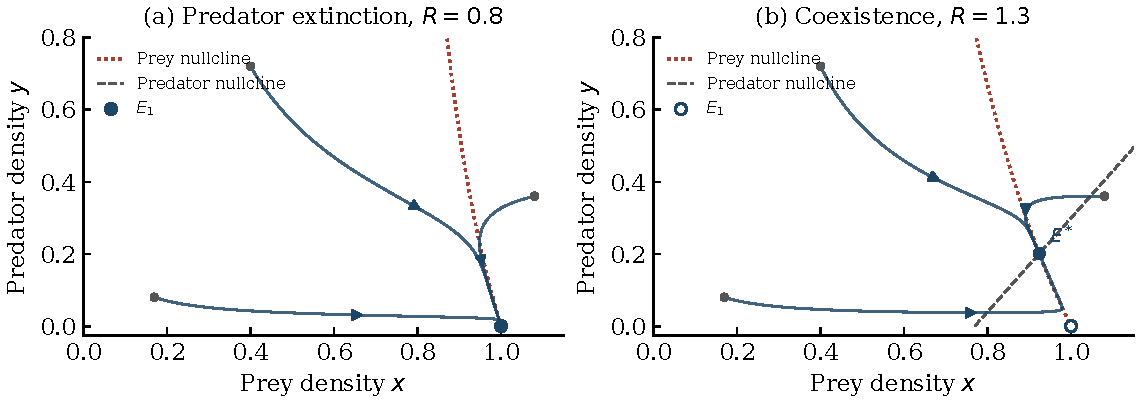
\includegraphics[width=\linewidth]{figures/num_invasion.pdf}
\caption{Phase portraits on the two sides of the invasion threshold, with the corresponding equilibrium and nullclines. Generated by \protect\path{code/numerical_study.py}.}
\label{fig:invasion}
\end{figure}

\subsection{Two stable coexistence states and a saddle boundary}
At \(m=3\) in the bistability case, the three feasible prey coordinates are approximately \(0.03542\), \(0.30000\) and \(0.56458\). The outer points attract, and the middle point is a saddle. In this case \(D=1.4\) exceeds \(M\chi(A)\simeq1.275\), so the basin theorem identifies the stable manifold as the common boundary. The starts \((0.12,14)\) and \((0.38,14)\) approach the low and high sinks, respectively. Figure~\ref{fig:basins} plots both trajectories and the boundary. The branch diagram varies \(m\) with the other inputs fixed, giving folds at \(m\simeq2.39552\) and \(m\simeq3.16069\).

\begin{figure}[!htbp]\centering
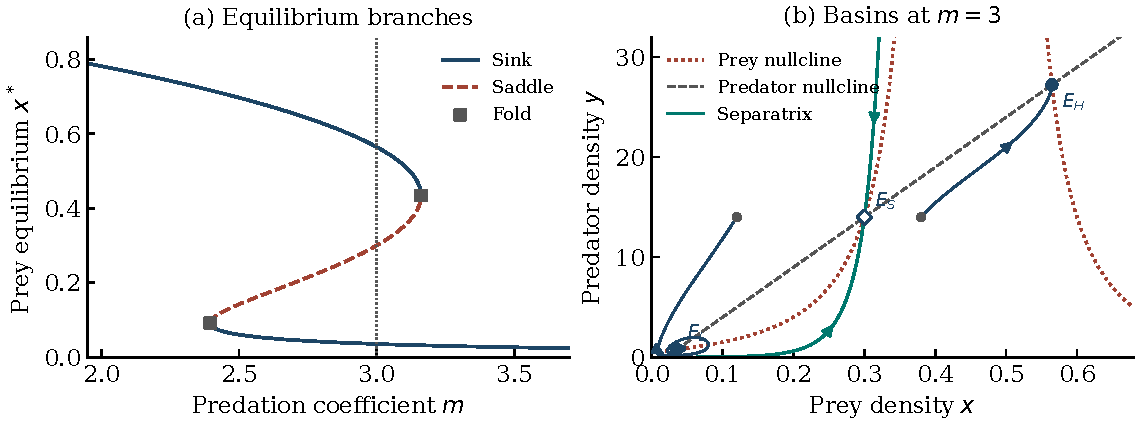
\includegraphics[width=\linewidth]{figures/num_basins.pdf}
\caption{Coexistence branches and phase portrait for the bistable case. The displayed separatrix is a numerical trace of the stable manifold of the middle saddle. Generated by \protect\path{code/numerical_study.py}.}
\label{fig:basins}
\end{figure}

\subsection{Predation and enrichment as Hopf parameters}
For the predation path the threshold is \(m_H=24/5\) at \((x^*,y^*)=(1/5,6/25)\). Its determinant is \(7/5\), its along-branch trace derivative is \(61/168\), and the cubic coefficient in the original-time convention is \(-1525/168\). For the enrichment path, \(k_H=1\) at \((x^*,y^*)=(1/10,162/1855)\). The corresponding values are \(49/25\), \(601/2520\) and \(-1415/252\). Both trace derivatives are positive and both cubic coefficients are negative. The crossings are supercritical. Figure~\ref{fig:hopf} shows phase portraits below and above each threshold. In the enrichment comparison only \(k\) varies, while \(\alpha\), \(m\), \(r\), \(\beta\), \(e\) and \(d\) remain fixed.

\begin{figure}[!htbp]\centering
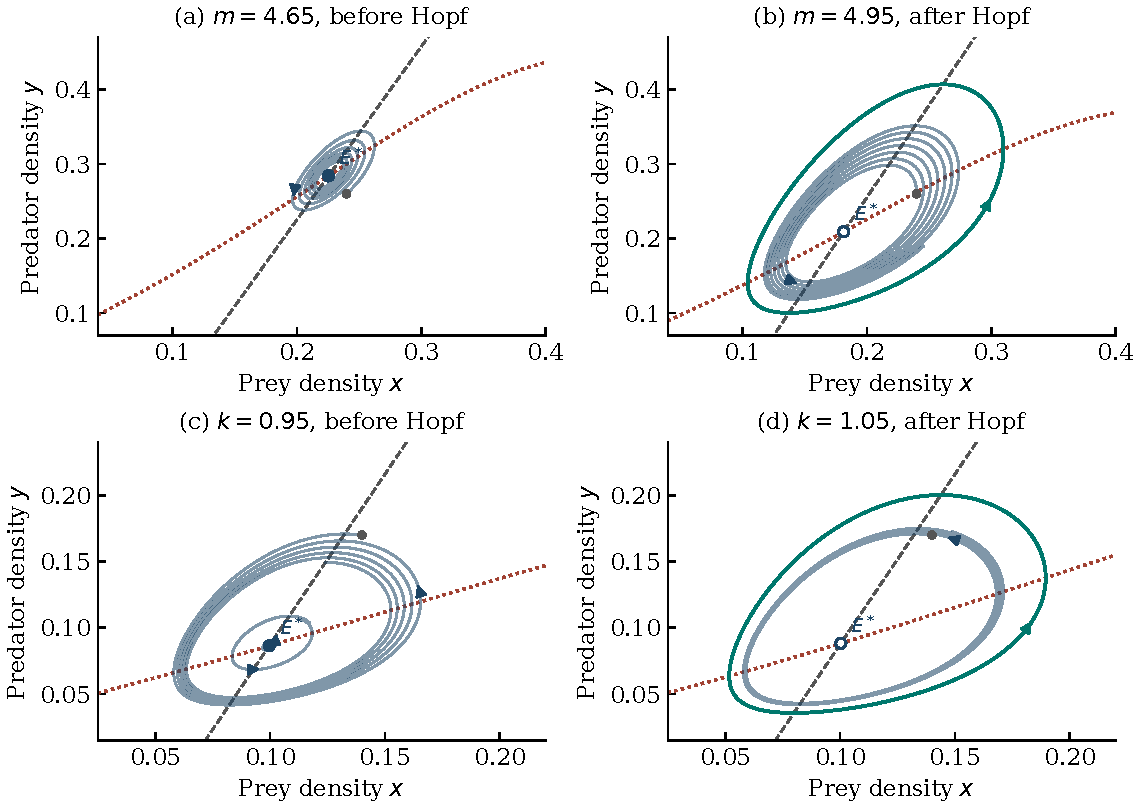
\includegraphics[width=\linewidth]{figures/num_hopf.pdf}
\caption{Phase portraits below and above the predation and enrichment Hopf thresholds. Thin lines show selected transient arcs. The green curve in the two cycling cases is the computed periodic orbit. Generated by \protect\path{code/numerical_study.py}.}
\label{fig:hopf}
\end{figure}

\subsection{Fold cusp and Bogdanov--Takens point}
The cusp in the \((m,\beta)\) plane is at \((3.7,4.5)\) for the inputs shown in Table~\ref{tab:constructed}. Its triple root is \(x^*=0.3\). Near it the fold curves separate regions with one and three feasible equilibria. For the Bogdanov--Takens example, \((m,k)=(17/5,1)\) and \((x^*,y^*)=(1/5,144/425)\). At the latter point \(Q=Q'=T=0\), the Jacobian has rank one, and the two quadratic normal-form coefficients are \(3\) and \(-13/12\). The unfolding determinant is \(-271/1224\). Figure~\ref{fig:two} displays the cusp folds and the local fold and trace-zero loci near the Bogdanov--Takens point. The trace-zero curve is shown where the determinant is positive. The regularity conditions also imply a local saddle-loop curve.

\begin{figure}[!htbp]\centering
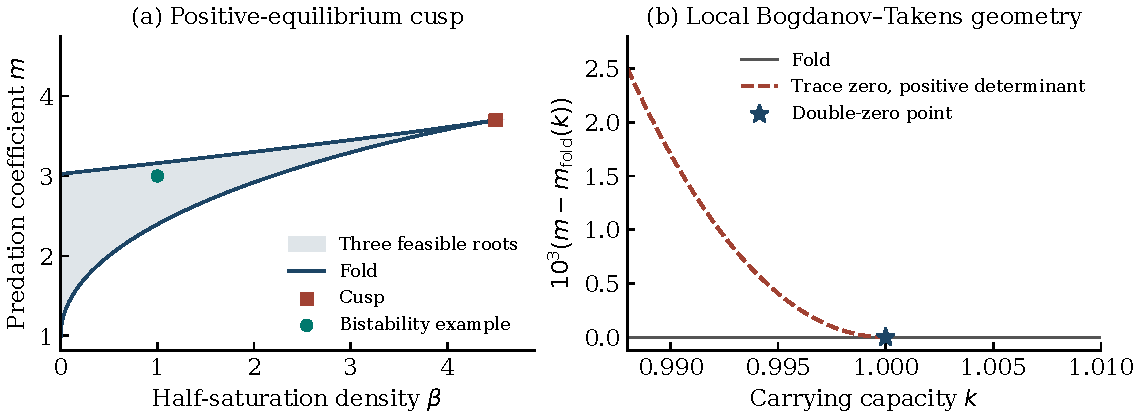
\includegraphics[width=\linewidth]{figures/num_two_parameters.pdf}
\caption{Two-parameter diagrams in the original model inputs. The cusp and the Bogdanov--Takens point arise on different parameter slices. Generated by \protect\path{code/numerical_study.py}.}
\label{fig:two}
\end{figure}

\subsection{A globally unique attracting orbit and a local cycle fold}
For the unique-cycle case \((A,M,R,D)=(10,12,5.5,3.5)\). The coexistence cubic strictly decreases on the strip, since \(p(X)+Xp'(X)\le3.7\) and \(M=12\). Its sole feasible root lies in \((0.21,0.27)\), where \(N>0\). Also \(M>\max p\). An exact Bernstein coefficient check of \(N'\mathcal Q-N\mathcal Q'\) on eight subintervals gives strict positivity on the full strip. The global uniqueness criterion therefore applies. Figure~\ref{fig:uniqueorbit} pairs the phase portrait with return diagnostics. The last section crossings from the three starts were within \(1.5\times10^{-7}\) of the computed crossing.

\begin{figure}[!htbp]\centering
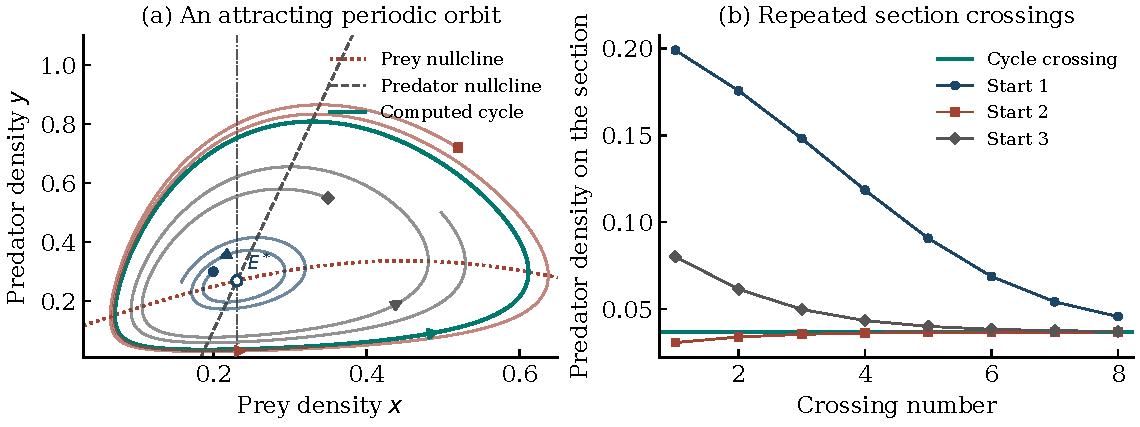
\includegraphics[width=\linewidth]{figures/num_cycle.pdf}
\caption{An attracting periodic orbit in the certified one-cycle region. A return-section calculation supplies the periodicity and attraction diagnostics. Generated by \protect\path{code/numerical_study.py}.}
\label{fig:uniqueorbit}
\end{figure}

Figure~\ref{fig:normalcycles} gives the separate local picture at supercritical Hopf and generalized Hopf. The generalized Hopf panel has two positive branches for \(-1/4<U<0\), one attracting and one repelling. The axes are scaled normal-form coordinates. Away from the organizing point, these curves do not give numerical amplitudes or a global count of periodic orbits for the population model.

\begin{figure}[!htbp]\centering
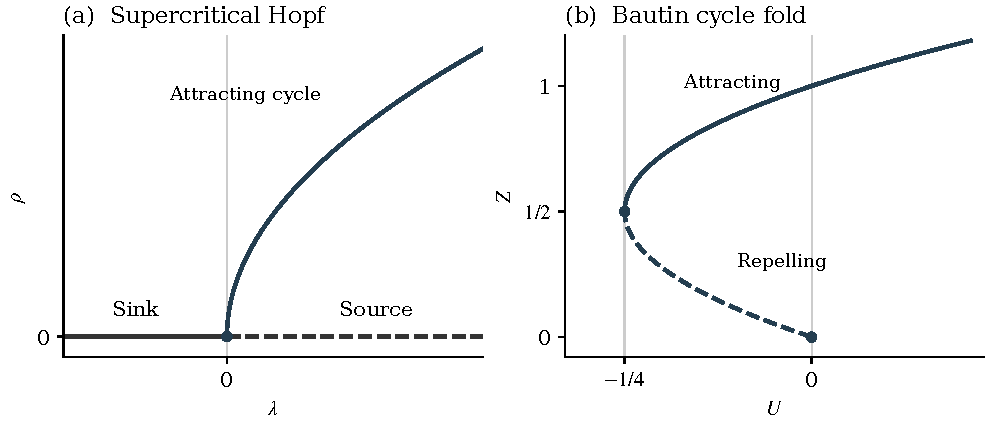
\includegraphics[width=\linewidth]{figures/analytical_cycles.pdf}
\caption{Local normal-form branches. At supercritical Hopf the stable cycle satisfies \(\rho^2=\lambda\). Near the generalized Hopf point the scaled cycle fold is \(U=Z^2-Z\). Solid branches are attracting and dashed branches repelling in the radial equation. Generated by \protect\path{code/analytical_diagram.py}.}
\label{fig:normalcycles}
\end{figure}

For a finite orbit calculation near the Bautin point, set \(r=k=\beta=1\), \(A=10\), \(s=0.1\), \(h_*=522/449+0.01\), and \(D=D_H+2\times10^{-5}\) in the Hopf family of Section~\ref{sec:family}. Then \(m\simeq3.335072\), \(e\simeq8.449066\) and \(d\simeq1.296992\). The low-density equilibrium is a stable focus. The directed return displacement on \(x=s\) changes sign in each of two disjoint brackets. Shooting gives an inner repelling orbit and an outer attracting orbit around this equilibrium. Figure~\ref{fig:bautin-numerical} shows the local configuration. A second stable focus and a saddle at higher prey densities lie outside the displayed region.

\begin{figure}[!htbp]\centering
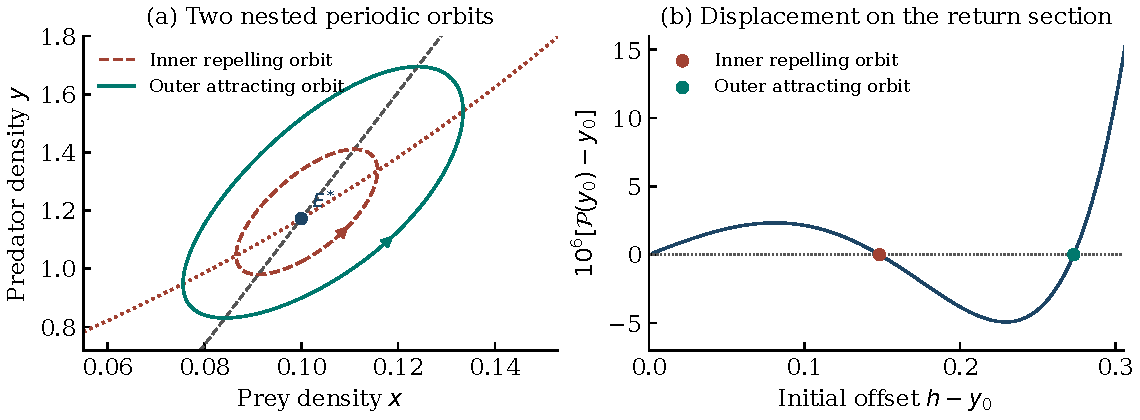
\includegraphics[width=\linewidth]{figures/num_bautin.pdf}
\caption{Two nested periodic orbits near generalized Hopf. The zeros of the return displacement correspond to the two curves in the phase plane. Here \(h\) in the axis label is the scaled predator equilibrium \(h_*\). Generated by \protect\path{code/numerical_study.py}.}
\label{fig:bautin-numerical}
\end{figure}

\begin{table}[!htbp]\centering
\caption{Periods and transverse multipliers at the computed periodic orbits. Every orbit closes to within \(1.3\times10^{-12}\) in the infinity norm after an independent Radau integration over its computed period.}
\label{tab:periods}
\begin{tabular}{@{}lrrl@{}}\toprule
Case & Period & Multiplier & Transverse stability\\ \midrule
Predation at \(m=4.95\) & 5.142344 & 0.79269272 & Attracting\\
Enrichment at \(k=1.05\) & 4.676835 & 0.94531264 & Attracting\\
Unique cycle & 2.882901 & 0.47852131 & Attracting\\
Bautin inner & 8.259431 & 1.00006672 & Repelling\\
Bautin outer & 8.381396 & 0.99973106 & Attracting\\
\bottomrule\end{tabular}
\end{table}

\subsection{Literature-informed prey growth rates}\label{sec:literature-cases}
Following \citet[Sec.~4, Table~6]{haque11}, we use the prey growth rates attributed to
\citet{tanner75}. Table~\ref{tab:lit-rates} separates the reported observed rates from
Tanner's estimates for optimal conditions. For all three species pairs we use
\(k=100,\ \alpha=0.04,\ m=1.20,\ \beta=10,\ e=0.25,\ d=0.30\), with time in years.
The choices of \(k\) and \(d\) match values used in Haque's numerical setup. The other
common inputs define a controlled comparison for Eq.~\eqref{eq:ode}. Tanner's predator
growth rates describe population increase and do not enter the mortality parameter \(d\).

\begin{table}[htbp]
\centering\small
\caption{Prey growth-rate intervals and results at the lower observed endpoint. Rate intervals
and the largest eigenvalue real part are in \(\mathrm{yr}^{-1}\). Tanner's maximum estimates
represent optimal conditions.}\label{tab:lit-rates}
\begin{tabular}{@{}lccccc@{}}
\toprule
Prey / predator & Observed & Maximum & \((x^*,y^*)\) & \(\max\Re\lambda\) & Type \\
\midrule
Muskrat / mink & 0.806--1.068 & 1.101--1.366 & (65.009, 55.009) & \(-0.30939\) & Node \\
Moose / wolf & 0.100--0.127 & 0.171--0.202 & (11.200, 1.200) & \(-0.00429\) & Focus \\
Snowshoe hare / lynx & 0.545--0.810 & 0.769--1.033 & (34.207, 24.207) & \(-0.08160\) & Focus \\
\bottomrule
\end{tabular}
\end{table}

The common inputs give \(R=10\), \(C=12\), \(C_{\rm crit}=6.25r\), and
\(d-m\chi(4)=0.06\). At the largest listed rate \(C_{\rm crit}=8.5375\), so the
unique-root and cycle-exclusion conditions guarantee global convergence throughout all
six intervals. The phase portraits in Fig.~\ref{fig:lit-rates} show a node for
muskrat/mink and damped oscillations for the other pairs at the lower observed rates.
The moose/wolf trajectory returns much more slowly at its lower rate. These comparisons
isolate the effect of \(r\) under the common inputs. The rate sweep includes both stable
nodes and stable foci in the observed hare interval. The remaining coefficients and initial
conditions are illustrative, so the trajectories give no estimates of wild population dynamics.

\begin{figure}[htbp]
\centering
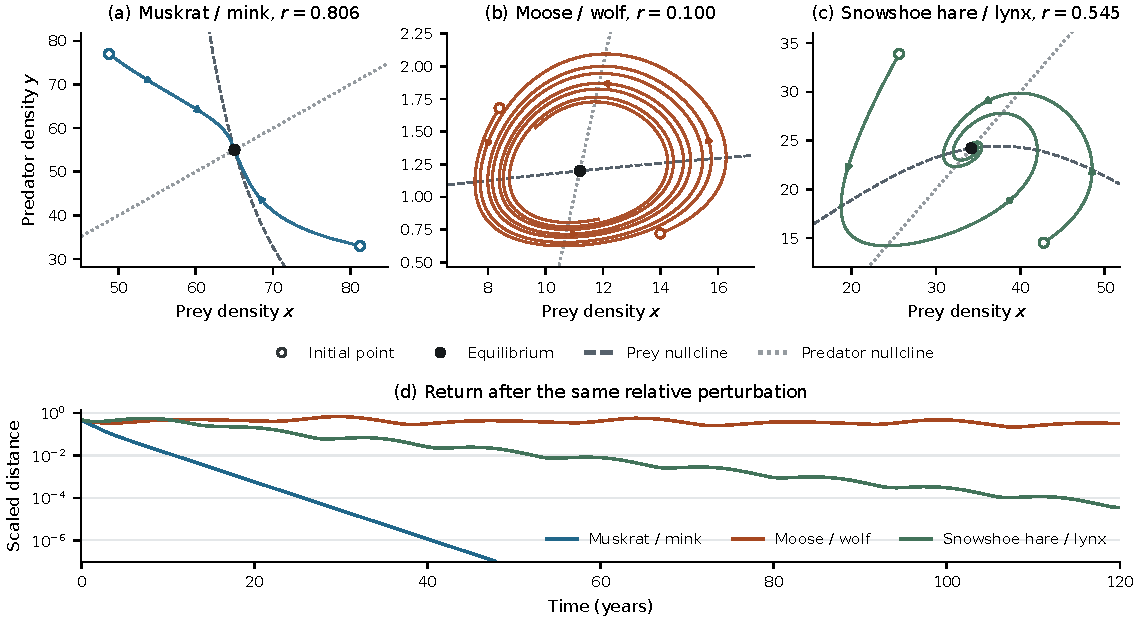
\includegraphics[width=\linewidth]{figures/lit_growth_rates.pdf}
\caption{Growth-rate comparison. Panels (a)--(c) use two initial points,
\((0.75x^*,1.4y^*)\) and \((1.25x^*,0.6y^*)\). Panel (d) shows the Euclidean distance in
\((x/x^*,y/y^*)\) from \((1,1)\) for the first initial point. The time span shown is
120 years. Python source \protect\texttt{code/literature\_cases.py}.}\label{fig:lit-rates}
\end{figure}

\FloatBarrier
